\documentclass[a4paper,12pt]{article}

% ---------- Pacotes ----------
\usepackage[utf8]{inputenc}
\usepackage[portuguese]{babel}
\usepackage[margin=1in]{geometry}

\usepackage{graphicx}
\usepackage{float}
\usepackage{subcaption}
\usepackage{caption}

\usepackage{amsmath}
\usepackage{amssymb}

\usepackage{booktabs}
\usepackage{array}
\usepackage{multirow}
\usepackage{makecell}

\usepackage{xcolor}
\usepackage{setspace}
\usepackage{indentfirst}
\usepackage{hyperref}

\usepackage{chngcntr}
\counterwithout{table}{section}

% ---------- Documento ----------
\begin{document}

% ---------- Capa ----------
\pagenumbering{gobble}
\begin{center}
    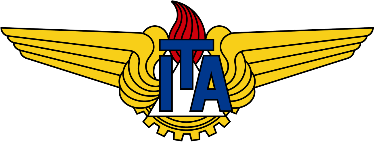
\includegraphics[width=0.5\linewidth]{images/ITA.png}\\[1cm]
    {\LARGE \textbf{Instituto Tecnológico de Aeronáutica}}\\[0.5cm]
    {\large \textbf{Divisão de Engenharia Aeronáutica}}\\[3cm]
    {\Large \textbf{PRJ-23 -- Projeto Preliminar de Aeronave}}\\[0.5cm]
    {\Large \textbf{Laboratório 04 -- Análise Aerodinâmica}}\\[0.5cm]
    {\Large \textbf{Equipe Ararinha Voadora}}\\[3cm]
\end{center}

\begin{flushleft}
    {\large \textbf{Alunos:}}\\
    {\normalsize Fabio Eiiti Kobayashi Urio}\\
    {\normalsize José Gilvan Alves dos Santos Junior}\\
    {\normalsize Pedro Antônio Cavalcante Teles}\\
    {\normalsize Rafael Fernandes Rosa}\\
    {\normalsize Vinycius Gabrihel Melo de Souza}\\
    {\normalsize William Daniel Da Paz Ferreira}\\[1.8cm]
\end{flushleft}

\begin{flushleft}
    {\large \textbf{Professor:}}\\
    {\normalsize Ney Rafael Sêcco}\\[3cm]
\end{flushleft}

\begin{center}
    {\Large 2026}
\end{center}
\newpage

\pagenumbering{arabic}

% ---------- Seções ----------
\newpage
\section{Modelagem da aeronave no AVL}

A aeronave da equipe foi modelada no AVL em dois arquivos de entrada,
\texttt{fwd.avl} e \texttt{aft.avl}, que compartilham a mesma geometria e
diferem apenas na posição do centro de gravidade usada como referência de
momentos. Toda a geometria foi extraída diretamente da configuração
convergida do \texttt{designTool}, o que garante consistência com os
trabalhos anteriores da equipe.

\begin{table}[H]
\centering
\caption{Cabeçalho dos arquivos de entrada do AVL.}\label{tab:avl_header}
\renewcommand{\arraystretch}{1.25}
\begin{tabular}{lcl}
\toprule
Parâmetro & Valor & Descrição \\
\midrule
$S_{\mathrm{ref}}$ & 368,833 & Área de referência [m$^2$] \\
$c_{\mathrm{ref}}$ & 6,8995 & Corda média aerodinâmica [m] \\
$b_{\mathrm{ref}}$ & 60,1518 & Envergadura de referência [m] \\
$X_{\mathrm{ref}}$ (\texttt{fwd.avl}) & 26,0772 & CG dianteiro [m] (15,4\,\%MAC) \\
$X_{\mathrm{ref}}$ (\texttt{aft.avl}) & 27,7190 & CG traseiro [m] (39,2\,\%MAC) \\
$C_{Dp}$ & 0,01489 & $C_{D0}$ por áreas molhadas do \texttt{designTool} \\
\bottomrule
\end{tabular}
\end{table}

A asa usa os perfis otimizados no Lab 03 (família do roteiro), aplicados por
\texttt{AFILE} nas estações de referência daquele trabalho, $\eta = 0{,}101$
(raiz), $\eta = 0{,}398$ (meio) e $\eta = 0{,}90$ (ponta). O perfil da raiz é
estendido até o plano de simetria e o da ponta até $\eta = 1$. Os arquivos de
coordenadas foram reamostrados de 321 para 197 pontos por limitação do
executável fornecido, sem perda prática porque o AVL extrai apenas a linha de
arqueamento. As empenagens usam NACA 0010, coerente com a espessura relativa
de 10\% definida no Lab 02. O fator \texttt{CLAF} foi mantido unitário em
todas as seções e o arrasto viscoso entra somente pelo $C_{Dp}$ do cabeçalho,
que recebe o $C_{D0}$ por áreas molhadas calculado pelo \texttt{designTool}
no ponto de projeto.

Três superfícies de controle foram definidas. O aileron ocupa 27\% da corda
entre $\eta = 0{,}56$ e $\eta = 0{,}90$, fechando a fração de envergadura de
34\% definida no Lab 02. O profundor e o leme têm charneira em 70\% da corda
das respectivas empenagens. A incidência da empenagem horizontal é a variável
de projeto \texttt{it} do AVL, usada nos ajustes de trimagem. A fuselagem, as
naceles e o winglet não são modelados, como no exemplo
\texttt{b737simple.avl} do material de aula.

\subsection*{Verificação da geometria}

A geometria construída pelo AVL foi conferida contra o \texttt{designTool}
pelas áreas que o próprio programa integra sobre os painéis
(Tabela~\ref{tab:avl_check}). O desvio de 0,55\% na asa corresponde à área
real medida ao longo do diedro de $6^\circ$, enquanto a área projetada
coincide exatamente com o trapézio do \texttt{designTool}. O mesmo vale para
a empenagem horizontal com seu diedro de $2^\circ$.

\begin{table}[H]
\centering
\caption{Verificação da geometria do AVL contra o \texttt{designTool}.}\label{tab:avl_check}
\renewcommand{\arraystretch}{1.25}
\begin{tabular}{lccc}
\toprule
Grandeza & \texttt{designTool} & AVL & Desvio \\
\midrule
Área da asa [m$^2$] & 368,833 & 370,864 & $+0{,}55\%$ (diedro) \\
Área da EH [m$^2$] & 64,546 & 64,584 & $+0{,}06\%$ (diedro) \\
Área da EV [m$^2$] & 61,472 & 61,472 & exato \\
Corda média geométrica da asa [m] & 6,1317 & 6,132 & exato \\
Corda média geométrica da EH [m] & 3,7459 & 3,746 & exato \\
\bottomrule
\end{tabular}
\end{table}

\newpage
\section{Ponto de projeto}

Adotou-se o mesmo ponto de projeto do Lab 03, a condição de cruzeiro com o
peso médio da fase, $W = 229\,669{,}3$ kgf, que corresponde a cerca de 44\%
da capacidade de combustível com 100\% de carga paga. A escolha mantém o
$C_L$ de projeto igual ao usado na otimização dos perfis, de modo que as
análises deste trabalho avaliam a asa exatamente na condição para a qual as
seções foram desenhadas. A Tabela~\ref{tab:ponto_projeto} reúne os dados
pedidos no roteiro.

\begin{table}[H]
\centering
\caption{Dados do ponto de projeto.}\label{tab:ponto_projeto}
\renewcommand{\arraystretch}{1.25}
\begin{tabular}{lcl}
\toprule
Parâmetro & Valor & Explicação \\
\midrule
$W_0$ & 2.857.571 & Peso máximo de decolagem da aeronave [N] \\
$W$ & 2.253.056 & Peso da aeronave no ponto de projeto [N] \\
$h$ & 10.668 & Altitude no ponto de projeto [m] \\
$\rho_\infty$ & 0,38046 & Densidade do ar no ponto de projeto [kg/m$^3$] \\
$a_\infty$ & 296,587 & Velocidade do som no ponto de projeto [m/s] \\
$M$ & 0,85 & Mach no ponto de projeto \\
$V$ & 252,1 & Velocidade no ponto de projeto [m/s] \\
$C_L$ & 0,5053 & $C_L$ no ponto de projeto \\
$S_{\mathrm{ref}}$ & 368,833 & Área de referência [m$^2$] \\
\bottomrule
\end{tabular}
\end{table}

O coeficiente de sustentação segue diretamente do equilíbrio vertical na
condição de cruzeiro:
\begin{equation*}
    C_L = \frac{W}{\tfrac{1}{2}\,\rho_\infty\,V^2\,S_{\mathrm{ref}}}
        = 0{,}5053.
\end{equation*}
Este é o valor usado como meta de sustentação (\texttt{a c 0.5053}) em todas
as simulações de cruzeiro do AVL neste relatório.

\newpage
\section{Validação da malha de vórtices}

Antes das análises, verificou-se que a discretização escolhida para o modelo
é suficiente. Todas as superfícies foram refinadas simultaneamente em seis
níveis, com totais de cerca de 100 a 2.000 vórtices, mantendo as proporções
entre asa e empenagens. Uma sétima malha, quatro vezes mais fina que a
adotada, foi executada apenas para servir de referência no cálculo dos
desvios. Cada nível rodou na condição do ponto de projeto, com $M = 0{,}85$
e meta de sustentação $C_L = 0{,}5053$. As métricas acompanhadas cobrem as
famílias de resultados usadas neste relatório: o ângulo de ataque de
equilíbrio, a derivada $C_{L\alpha}$, o arrasto induzido e a posição do
ponto neutro.

\begin{table}[H]
\centering
\caption{Convergência de malha na condição do ponto de projeto.}\label{tab:convergencia}
\renewcommand{\arraystretch}{1.25}
\begin{tabular}{ccccccc}
\toprule
Malha da asa & Vórtices & $\alpha$ [graus] & $C_{L\alpha}$ [1/rad] &
$C_{D,\mathrm{ind}}$ & $C_{D,\mathrm{ff}}$ (Trefftz) & $x_{np}$ [m] \\
\midrule
$3\times 12$ & 110 & 3,9041 & 6,4022 & 0,01057 & 0,00925 & 29,9379 \\
$5\times 16$ & 217 & 3,8870 & 6,4288 & 0,01063 & 0,00924 & 30,0270 \\
$8\times 25$ & 532 & 3,8741 & 6,4584 & 0,01019 & 0,00919 & 30,0547 \\
$10\times 35$ & 966 & 3,8823 & 6,4533 & 0,01022 & 0,00924 & 30,0634 \\
$12\times 40$ (adotada) & 1.312 & 3,8752 & 6,4626 & 0,01014 & 0,00923 & 30,0651 \\
$15\times 50$ & 2.050 & 3,8720 & 6,4697 & 0,01015 & 0,00922 & 30,0703 \\
$24\times 80$ (referência) & 5.248 & 3,8700 & 6,4737 & 0,00991 & 0,00923 & 30,0776 \\
\bottomrule
\end{tabular}
\end{table}

\begin{figure}[H]
\centering
\caption{Desvio percentual das métricas em relação à malha de referência
($24\times 80$), em escala logarítmica. A linha tracejada marca a malha
adotada.}\label{fig:convergencia}
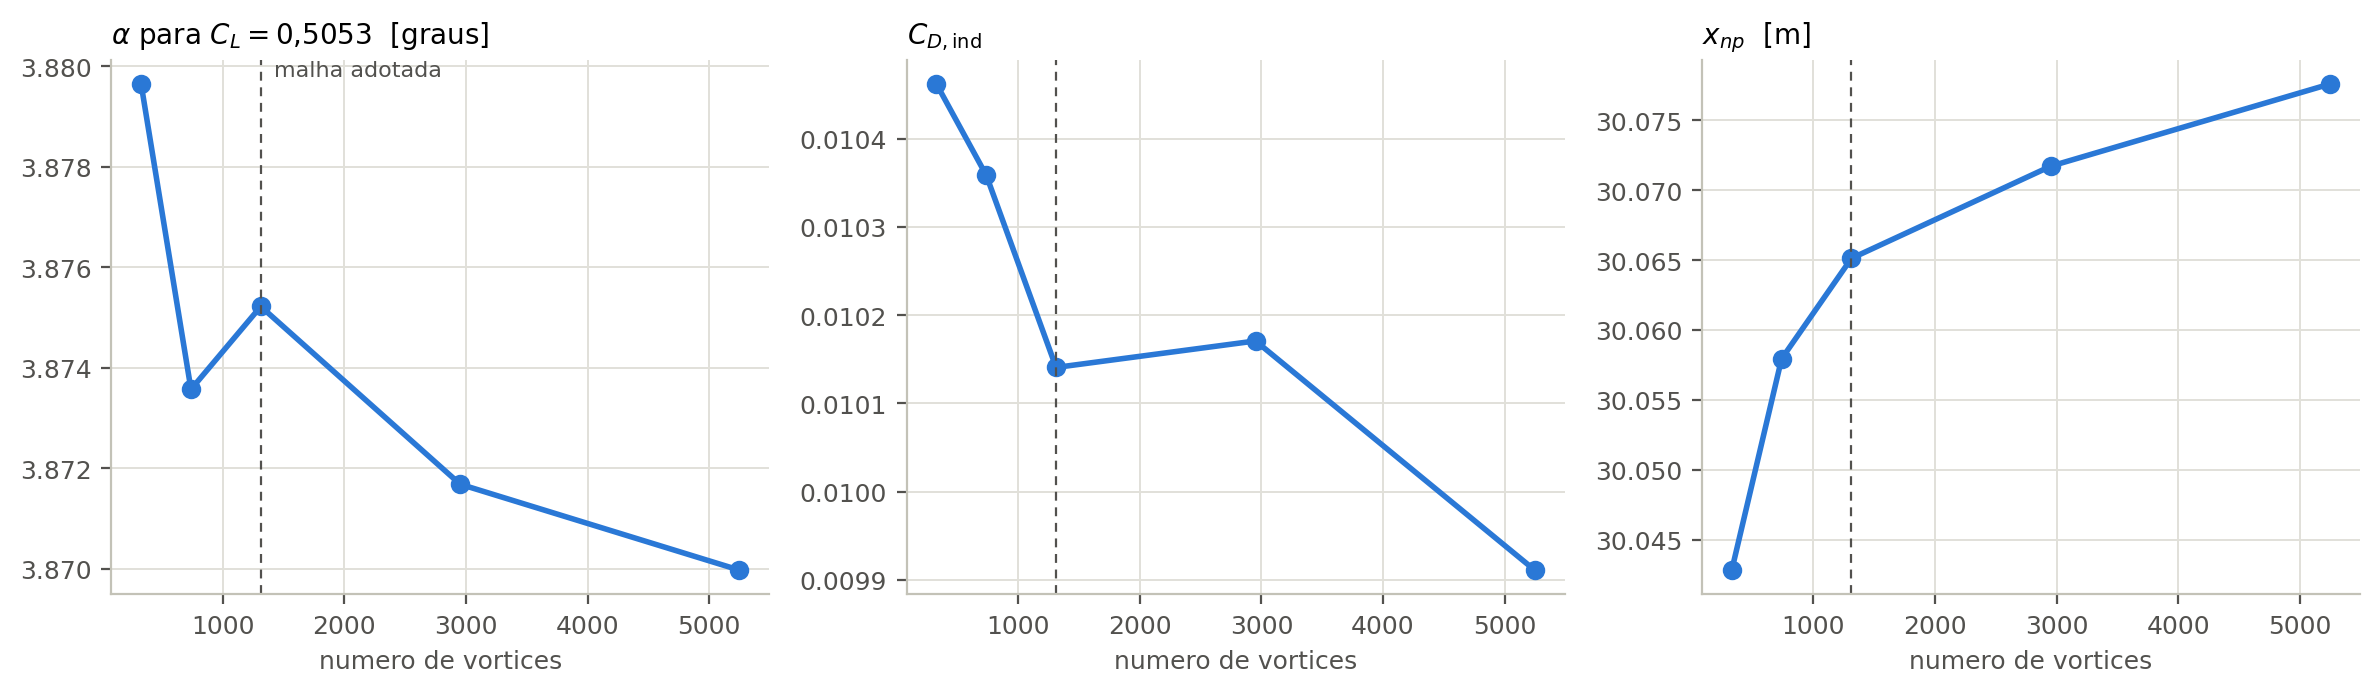
\includegraphics[width=\linewidth]{images/03_convergencia/convergencia_malha.png}
\end{figure}

A Figura~\ref{fig:convergencia} apresenta o desvio percentual em relação à
malha de referência das três métricas que exibem transiente de convergência
na faixa varrida. As três caem de forma consistente com o refino, de cerca
de 1\% na malha mais grossa para menos de 0,1\% na mais fina. Na malha
adotada, o ângulo de ataque difere da referência em 0,14\%, a derivada
$C_{L\alpha}$ em 0,17\% e o ponto neutro em 0,04\%, o que corresponde a
3,5~cm ou 0,05\,\%MAC.

O arrasto induzido do plano de Trefftz, que é a medida limpa do método, já
parte convergido: varia menos de 0,5\% em toda a varredura e a malha
adotada difere da referência em 0,01\% (Tabela~\ref{tab:convergencia}). A
integração de campo próximo oscila numa banda de cerca de 2\% sem tendência
com o refino, comportamento conhecido dessa forma de cálculo, e por isso a
curva de Trefftz é a referência para julgar o arrasto. Refinos além de
2.000 vórtices foram avaliados e os desvios apenas flutuam num piso de
ruído abaixo de 0,15\%, sem queda sistemática, o que confirma que a
varredura apresentada cobre toda a região de interesse.

A malha adotada nos arquivos da entrega, com $12\times 40$ painéis na asa e
1.312 vórtices no total, foi portanto considerada convergida para os
propósitos deste trabalho, com custo compatível com as rodadas interativas
exigidas pelo roteiro.

\newpage
\section{Incidência da empenagem horizontal}

A incidência da empenagem horizontal de cada configuração foi ajustada para
anular a deflexão de profundor na condição de cruzeiro. Em cada arquivo
fixou-se a meta de sustentação do ponto de projeto ($M = 0{,}85$,
$C_L = 0{,}5053$) e a restrição de momento de arfagem nulo pelo profundor.
Como a resposta $\delta_e(i_t)$ é linear no método de malha de vórtices, o
zero foi resolvido com duas avaliações e uma rodada de verificação,
resultando em deflexões residuais abaixo de $0{,}01^\circ$, uma ordem de
grandeza melhor que a tolerância de $0{,}1^\circ$ sugerida no roteiro. A
Tabela~\ref{tab:trimagem} resume os resultados para a asa final, com a
torção otimizada da Seção~\ref{sec:torcao}.

\begin{table}[H]
\centering
\caption{Incidência da empenagem que anula a deflexão de profundor em cruzeiro.}\label{tab:trimagem}
\renewcommand{\arraystretch}{1.25}
\begin{tabular}{lccc}
\toprule
Configuração & $i_t$ [graus] & $\delta_e$ residual [graus] & $\alpha$ [graus] \\
\midrule
CG dianteiro (\texttt{fwd.avl}) & $-4{,}48$ & $-0{,}001$ & 5,38 \\
CG traseiro (\texttt{aft.avl}) & $-1{,}98$ & $+0{,}0004$ & 5,07 \\
\bottomrule
\end{tabular}
\end{table}

As incidências resultantes ficaram próximas da faixa de um transporte
convencional, que tipicamente opera com estabilizador entre $-3^\circ$ e
$+1^\circ$, com a torção da asa aliviando cerca de $4{,}0^\circ$ em
relação à asa sem torção, um dos ganhos da otimização da Seção 6. A
magnitude residual, ainda algo alta no CG dianteiro, tem dois fatores.
Primeiro, a fuselagem não é modelada no AVL, o que desloca o ponto neutro
para trás e infla a margem estática, exigindo mais força de compensação da
empenagem. Segundo, os perfis supercríticos otimizados no Lab 03 têm
momento de arfagem fortemente negativo, que precisa ser equilibrado pela
cauda. A validação do ajuste aparece nas polares da
Seção~\ref{sec:polares}: nas curvas de $C_L \times \delta_e$ os casos
compensados cruzam $\delta_e = 0$ exatamente no $C_L$ de projeto.

\newpage
\section{Método da seção crítica}\label{sec:secao_critica}

O $C_{L\mathrm{max}}$ de asa limpa em baixa velocidade foi determinado pelo
método da seção crítica em $M = 0{,}2$, com a incidência de empenagem de
cruzeiro da seção anterior. Para cada posição de CG, com e sem a restrição
de trimagem, o ângulo de ataque foi aumentado até a distribuição de
coeficiente de sustentação local da asa, no plano normal ao enflechamento
(\texttt{cl\_norm} do AVL), alcançar o limite de $c_{\ell\mathrm{max}}$ dos
perfis otimizados. O limite usado é o do Lab 03 no plano normal, com a
correção da calibração do XFoil: 1,774 na raiz, 1,799 no meio e 1,734 na
ponta, interpolado linearmente entre as estações. Como o método é linear, o
cruzamento foi resolvido por interpolação na varredura de $\alpha$.

Uma primeira aplicação do método na asa sem torção revelou estol começando
na ponta, em $\eta = 0{,}89$, sobre a região do aileron, com
$C_{L\mathrm{max}}$ entre 0,83 e 0,92. Esse diagnóstico motivou a
otimização de torção apresentada na Seção 6, e os resultados a seguir
referem-se à asa final, já com a torção aplicada.

\begin{table}[H]
\centering
\caption{Resultados do método da seção crítica para os quatro casos, asa final.}\label{tab:secao_critica}
\renewcommand{\arraystretch}{1.25}
\begin{tabular}{lccc}
\toprule
Caso & $\alpha_{\mathrm{max}}$ [graus] & $C_{L\mathrm{max}}$ & $\delta_e$ [graus] \\
\midrule
CG dianteiro sem trimagem & 14,72 & 1,130 & 0,0 \\
CG dianteiro com trimagem & 14,77 & 1,036 & $-17{,}07$ \\
CG traseiro sem trimagem & 14,70 & 1,155 & 0,0 \\
CG traseiro com trimagem & 14,73 & 1,097 & $-10{,}70$ \\
\bottomrule
\end{tabular}
\end{table}

\begin{figure}[H]
\centering
\caption{Distribuições de coeficiente de sustentação da asa na condição de
estol, com a curva limite de $c_{\ell\mathrm{max}}$ dos perfis. A estrela
marca a seção crítica.}\label{fig:clxy}
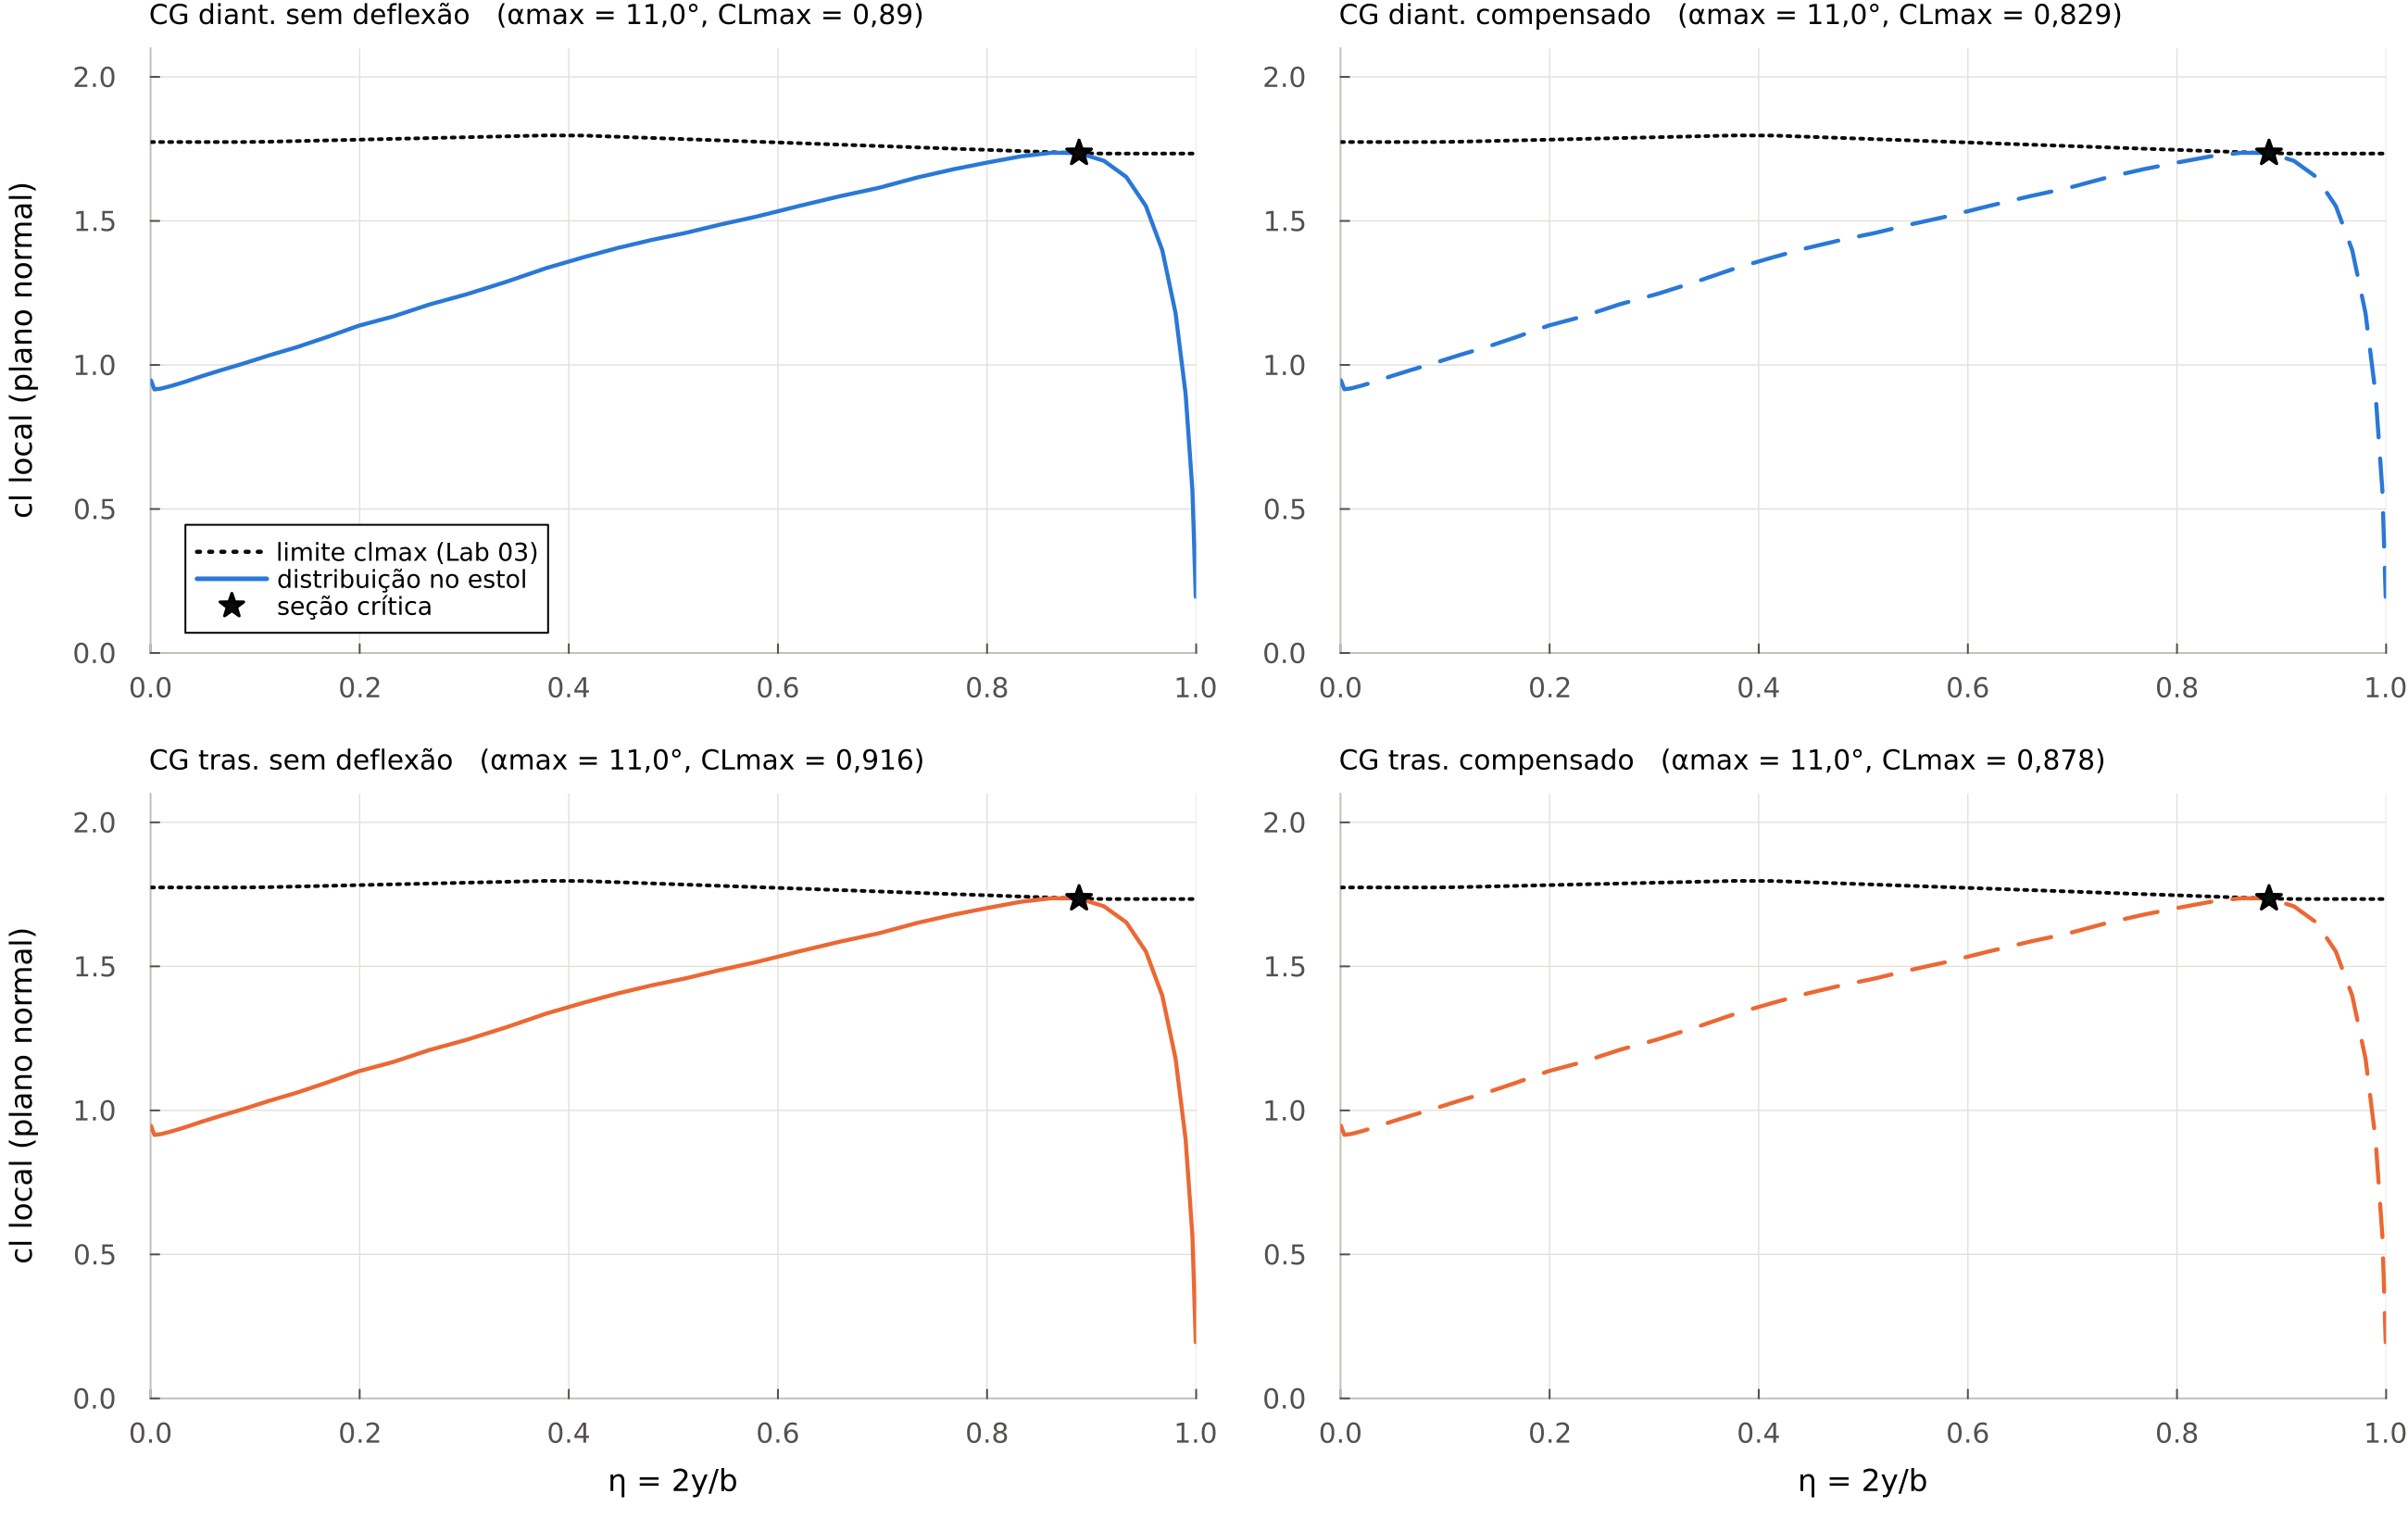
\includegraphics[width=\linewidth]{images/05_secao_critica/clxy_estol.png}
\end{figure}

O ângulo de estol é praticamente o mesmo nos quatro casos, em torno de
$14{,}7^\circ$, porque a distribuição de sustentação da asa quase não muda
com o CG ou com a trimagem. O que muda é o $C_{L\mathrm{max}}$ da
aeronave: a compensação exige força para baixo na empenagem, que subtrai
sustentação total, e o efeito é maior no CG dianteiro, onde o braço de
compensação é maior. O caso mais restritivo é o CG dianteiro com trimagem,
com $C_{L\mathrm{max}} = 1{,}036$.

\subsection*{Características de estol}

Com a torção otimizada, a seção crítica fica em $\eta = 0{,}45$ em todos
os casos: o estol começa na metade interna da asa, antes do aileron, que
ocupa de $\eta = 0{,}56$ a $\eta = 0{,}90$. A característica é adequada: a
separação inicial ocorre longe das superfícies de comando lateral e a
região da ponta mantém folga de sustentação, preservando o controle de
rolamento no início do estol.

Os valores de $C_{L\mathrm{max}}$, entre 1,04 e 1,16, ficam abaixo da
estimativa de asa limpa do \texttt{designTool}, de 1,33. Contribuem para a
diferença o limite de $c_{\ell\mathrm{max}}$ ser aplicado no plano normal,
o que equivale a um limite na direção da corrente cerca de 28\% menor, e o
desconto da força de compensação da empenagem, efeitos que a correlação
histórica do \texttt{designTool} não captura. A deflexão de profundor no
estol trimado do CG dianteiro, de $-17{,}1^\circ$, é alta mas permanece
dentro de batentes típicos de $\pm 25^\circ$.

\input{secoes/06-polares}
\newpage
\section{Ponto neutro e margem estática}

O ponto neutro foi obtido do comando \texttt{st} do AVL na condição do
ponto de projeto, com a incidência de empenagem trimada, resultando em
$x_{np} = 30{,}125$ m, ou 74,1\,\%MAC. As margens estáticas
correspondentes às duas posições de CG são
\begin{equation*}
    SM_{\mathrm{fwd}} = \frac{x_{np} - x_{cg,\mathrm{fwd}}}{c_{\mathrm{ref}}}
    = 58{,}7\,\%\mathrm{MAC},
    \qquad
    SM_{\mathrm{aft}} = \frac{x_{np} - x_{cg,\mathrm{aft}}}{c_{\mathrm{ref}}}
    = 34{,}9\,\%\mathrm{MAC}.
\end{equation*}

Os valores são bem maiores que os estimados pelo \texttt{designTool} no
Lab 02, que situa o ponto neutro em 45,4\,\%MAC, com margens de 30,0\% e
6,2\%. A diferença é esperada e tem origem na fuselagem, que não é
modelada no AVL. O momento desestabilizante do corpo desloca o ponto
neutro real para a frente, e o \texttt{designTool} contabiliza esse efeito
por correlação empírica. Para o projeto, a estimativa do
\texttt{designTool} é a conservadora, e as margens do AVL devem ser lidas
como as da combinação asa e empenagem isoladas. Essa mesma diferença
explica as incidências de trimagem elevadas da Seção 4 e sugere, como
próximo passo, incluir a fuselagem no modelo do AVL para as análises
finais de estabilidade.

\newpage
\section{Derivadas de estabilidade}

As derivadas foram levantadas para a configuração de CG traseiro
(\texttt{aft.avl}) no ponto de projeto, sem restrição de trimagem: meta de
sustentação $C_L = 0{,}5053$ em $M = 0{,}85$, profundor fixo em zero e
incidência de empenagem de cruzeiro ($i_t = -5{,}90^\circ$), o que resulta
em $\alpha = 4{,}60^\circ$. As derivadas longitudinais e de força lateral
vêm do comando \texttt{st} (eixos de estabilidade), os momentos
látero-direcionais do comando \texttt{sb} (eixos do corpo), e as derivadas
de arrasto em relação a $q$, $i_t$ e $\delta_e$ de diferenças finitas
centradas na mesma condição. Os dados gerais da aeronave estão na
Tabela~\ref{tab:dados_gerais}, com os momentos de inércia calculados pela
função auxiliar da disciplina com a fração de combustível de 44\% que
reproduz o peso do ponto de projeto e 100\% de carga paga.

\begin{table}[H]
\centering
\caption{Informações gerais para análise de estabilidade e controle.}\label{tab:dados_gerais}
\renewcommand{\arraystretch}{1.25}
\begin{tabular}{lcl}
\toprule
Parâmetro & Valor & Fonte \\
\midrule
$S_{\mathrm{ref}}$ [m$^2$] & 368,833 & \texttt{designTool} \\
$c_{\mathrm{ref}}$ [m] & 6,8995 & \texttt{designTool} \\
$b_{\mathrm{ref}}$ [m] & 60,1518 & \texttt{designTool} \\
$m$ [kg] & 229.669,3 & \texttt{designTool} \\
$I_{xx}$ [kg$\cdot$m$^2$] & $1{,}508\times 10^{7}$ & \texttt{designTool} \\
$I_{yy}$ [kg$\cdot$m$^2$] & $4{,}284\times 10^{7}$ & \texttt{designTool} \\
$I_{zz}$ [kg$\cdot$m$^2$] & $5{,}578\times 10^{7}$ & \texttt{designTool} \\
$I_{xz}$ [kg$\cdot$m$^2$] & $1{,}209\times 10^{6}$ & \texttt{designTool} \\
$i_p$ [graus] & 0,0 & \texttt{designTool} \\
$x_p$ [m] & 18,0 & \texttt{designTool} \\
$z_p$ [m] & 3,0 & \texttt{designTool}, sinal invertido para o MVO \\
$T_{\mathrm{max}}$ [N] & 1.026.000 & \texttt{designTool}, 513.000 por motor \\
$V$ [m/s] & 252,1 & ponto de projeto \\
$h$ [m] & 10.668 & ponto de projeto \\
\bottomrule
\end{tabular}
\end{table}

\subsection*{Resultados em $\alpha = 0$ e ajuste da polar}

O $C_{L0}$ e o $C_{M0}$ vêm de uma rodada com $\alpha = 0$, $i_t = 0$ e
profundor nulo. O ajuste quadrático $C_D = C_{D0} + C_{D\alpha}\,\alpha +
C_{D\alpha 2}\,\alpha^2$ foi feito sobre a polar não trimada do CG
traseiro (item 5.b), com $\alpha$ em radianos.

\begin{table}[H]
\centering
\caption{Resultados para $\alpha = 0$, $i_t = 0$ e ajuste quadrático da polar.}\label{tab:cl0_polar}
\renewcommand{\arraystretch}{1.25}
\begin{tabular}{lcl}
\toprule
Parâmetro & Valor & Fonte \\
\midrule
$C_{L0}$ & 0,0670 & AVL \texttt{ft} \\
$C_{M0}$ & $-0{,}1346$ & AVL \texttt{ft} \\
$C_{D0}$ & 0,01954 & ajuste do item 5.b \\
$C_{D\alpha}$ [1/rad] & $-0{,}0424$ & ajuste do item 5.b \\
$C_{D\alpha 2}$ [1/rad$^2$] & 1,5770 & ajuste do item 5.b \\
\bottomrule
\end{tabular}
\end{table}

\subsection*{Tabela completa de derivadas}

A Tabela~\ref{tab:derivadas} apresenta os valores lidos do AVL e os
valores finais para o MVO, já com as conversões do roteiro aplicadas: as
derivadas de controle ($i_t$, $\delta_e$, $\delta_a$ e $\delta_r$) foram
multiplicadas por $180/\pi$, e os sinais de $C_{Y\beta}$, $C_{Yp}$,
$C_{Yr}$, $C_{\ell\delta a}$, $C_{\ell\delta r}$, $C_{n\delta a}$ e
$C_{n\delta r}$ foram invertidos pela diferença de convenções.

\begin{table}[H]
\centering
\caption{Derivadas de estabilidade para o CG traseiro no ponto de projeto.}\label{tab:derivadas}
\renewcommand{\arraystretch}{1.15}
\begin{tabular}{lccl}
\toprule
Parâmetro & Valor AVL & Valor MVO & Fonte e conversão \\
\midrule
$C_{L\alpha}$ [1/rad] & 6,4672 & 6,4672 & \texttt{st} \\
$C_{Lq}$ [1/rad] & 10,8669 & 10,8669 & \texttt{st} \\
$C_{Lit}$ & 0,013865 & 0,7944 & \texttt{st}, $\times 180/\pi$ \\
$C_{L\delta e}$ & 0,007719 & 0,4423 & \texttt{st}, $\times 180/\pi$ \\
$C_{Dq}$ [1/rad] & 0,1535 & 0,1535 & dif. finita \\
$C_{Dit}$ & $-0{,}000170$ & $-0{,}0097$ & dif. finita, $\times 180/\pi$ \\
$C_{D\delta e}$ & $-0{,}000090$ & $-0{,}0052$ & dif. finita, $\times 180/\pi$ \\
$C_{M\alpha}$ [1/rad] & $-2{,}2551$ & $-2{,}2551$ & \texttt{st} \\
$C_{Mq}$ [1/rad] & $-32{,}4502$ & $-32{,}4502$ & \texttt{st} \\
$C_{Mit}$ & $-0{,}052910$ & $-3{,}0315$ & \texttt{st}, $\times 180/\pi$ \\
$C_{M\delta e}$ & $-0{,}030696$ & $-1{,}7588$ & \texttt{st}, $\times 180/\pi$ \\
$C_{Y\beta}$ [1/rad] & $-0{,}4029$ & 0,4029 & \texttt{st}, sinal invertido \\
$C_{Yp}$ [1/rad] & 0,0251 & $-0{,}0251$ & \texttt{st}, sinal invertido \\
$C_{Yr}$ [1/rad] & 0,4386 & $-0{,}4386$ & \texttt{st}, sinal invertido \\
$C_{Y\delta r}$ & $-0{,}004035$ & $-0{,}2312$ & \texttt{st}, $\times 180/\pi$ \\
$C_{\ell\beta}$ [1/rad] & $-0{,}2354$ & $-0{,}2354$ & \texttt{st} \\
$C_{\ell p}$ [1/rad] & $-0{,}5602$ & $-0{,}5602$ & \texttt{sb} \\
$C_{\ell r}$ [1/rad] & 0,1790 & 0,1790 & \texttt{sb} \\
$C_{\ell\delta a}$ & $-0{,}004157$ & 0,2382 & \texttt{sb}, sinal e $\times 180/\pi$ \\
$C_{\ell\delta r}$ & $-0{,}000505$ & 0,0289 & \texttt{sb}, sinal e $\times 180/\pi$ \\
$C_{n\beta}$ [1/rad] & 0,1735 & 0,1735 & \texttt{st} \\
$C_{np}$ [1/rad] & $-0{,}0905$ & $-0{,}0905$ & \texttt{sb} \\
$C_{nr}$ [1/rad] & $-0{,}2037$ & $-0{,}2037$ & \texttt{sb} \\
$C_{n\delta a}$ & $-0{,}000136$ & 0,0078 & \texttt{sb}, sinal e $\times 180/\pi$ \\
$C_{n\delta r}$ & 0,002190 & $-0{,}1255$ & \texttt{sb}, sinal e $\times 180/\pi$ \\
\bottomrule
\end{tabular}
\end{table}

Duas verificações de sanidade sustentam a tabela. A derivada $C_{Lq}$
obtida por diferença finita coincide com a do \texttt{st} em todas as
casas apresentadas, validando o procedimento numérico usado para as
derivadas de arrasto. E a relação $x_{np} = x_{cg} -
c_{\mathrm{ref}}\,C_{M\alpha}/C_{L\alpha}$ reproduz o ponto neutro da
Seção 7 com o $C_{M\alpha}$ e o $C_{L\alpha}$ da tabela.


\end{document}
